\documentclass[aspectratio=169,svgnames]{beamer}

\usepackage{lmodern}
\usepackage[T1]{fontenc}
\usepackage[ngerman]{babel}
\usepackage{selinput}
\SelectInputMappings{%
   adieresis={ä},
   germandbls={ß}
   }
\usepackage{csquotes}

\usepackage{hyperref}

\usepackage{listings}
\newcommand\YAMLcolonstyle{\color{red}\mdseries}
\newcommand\YAMLkeystyle{\color{black}\bfseries}
\newcommand\YAMLvaluestyle{\color{blue}\mdseries}

\makeatletter

% here is a macro expanding to the name of the language
% (handy if you decide to change it further down the road)
\newcommand\language@yaml{yaml}

\expandafter\expandafter\expandafter\lstdefinelanguage
\expandafter{\language@yaml}
{
  backgroundcolor=\color{Cornsilk}, 
  keywords={true,false,null,y,n},
  keywordstyle=\color{darkgray}\bfseries,
  basicstyle=\YAMLkeystyle,                                 % assuming a key comes first
  sensitive=false,
  comment=[l]{\#},
  morecomment=[s]{/*}{*/},
  commentstyle=\color{purple}\ttfamily,
  stringstyle=\YAMLvaluestyle\ttfamily,
  moredelim=[l][\color{orange}]{\&},
  moredelim=[l][\color{magenta}]{*},
  moredelim=**[il][\YAMLcolonstyle{:}\YAMLvaluestyle]{:},   % switch to value style at :
  morestring=[b]',
  morestring=[b]",
  literate =    {---}{{\ProcessThreeDashes}}3
                {>}{{\textcolor{red}\textgreater}}1     
                {|}{{\textcolor{red}\textbar}}1 
                {\ -\ }{{\mdseries\ -\ }}3,
}

% switch to key style at EOL
\lst@AddToHook{EveryLine}{\ifx\lst@language\language@yaml\YAMLkeystyle\fi}
\makeatother

\newcommand\ProcessThreeDashes{\llap{\color{cyan}\mdseries-{-}-}}

\usepackage{siunitx}
\DeclareSIUnit\inch{in}
\DeclareSIUnit\in{in}

\usetheme{Rochester}  %% Themenwahl

\setbeamercovered{transparent}
%\setbeamertemplate{footline}[frame number]
% \usecolortheme{spruce}        % grün
% \usecolortheme{beetle}
\usecolortheme{cormorant}
% \usecolortheme[named=MSUgreen]{structure}
\newcommand{\hshblogo}{\includegraphics[width=1.3cm]{space-logo}}
\newcommand{\divider}[1]{\begin{frame} %
\begin{alertblock}{} %
\centering\usebeamerfont{section title}#1 %
\end{alertblock} %
\end{frame}}

\title{Ein mobiler CO2 Sensor}
\author{Syralist}
\date{17.06.2025}
\logo{
\includegraphics[width=1.1cm]{Syralist_Kalligraphie_Logo_rund}}
 
\begin{document}
\maketitle
% \frame{\tableofcontents}

\begin{frame}%[<+->] %%Eine Folie
    \frametitle{Ich habe einen mobilen CO2 Sensor gebaut} %%Folientitel
    \centering
    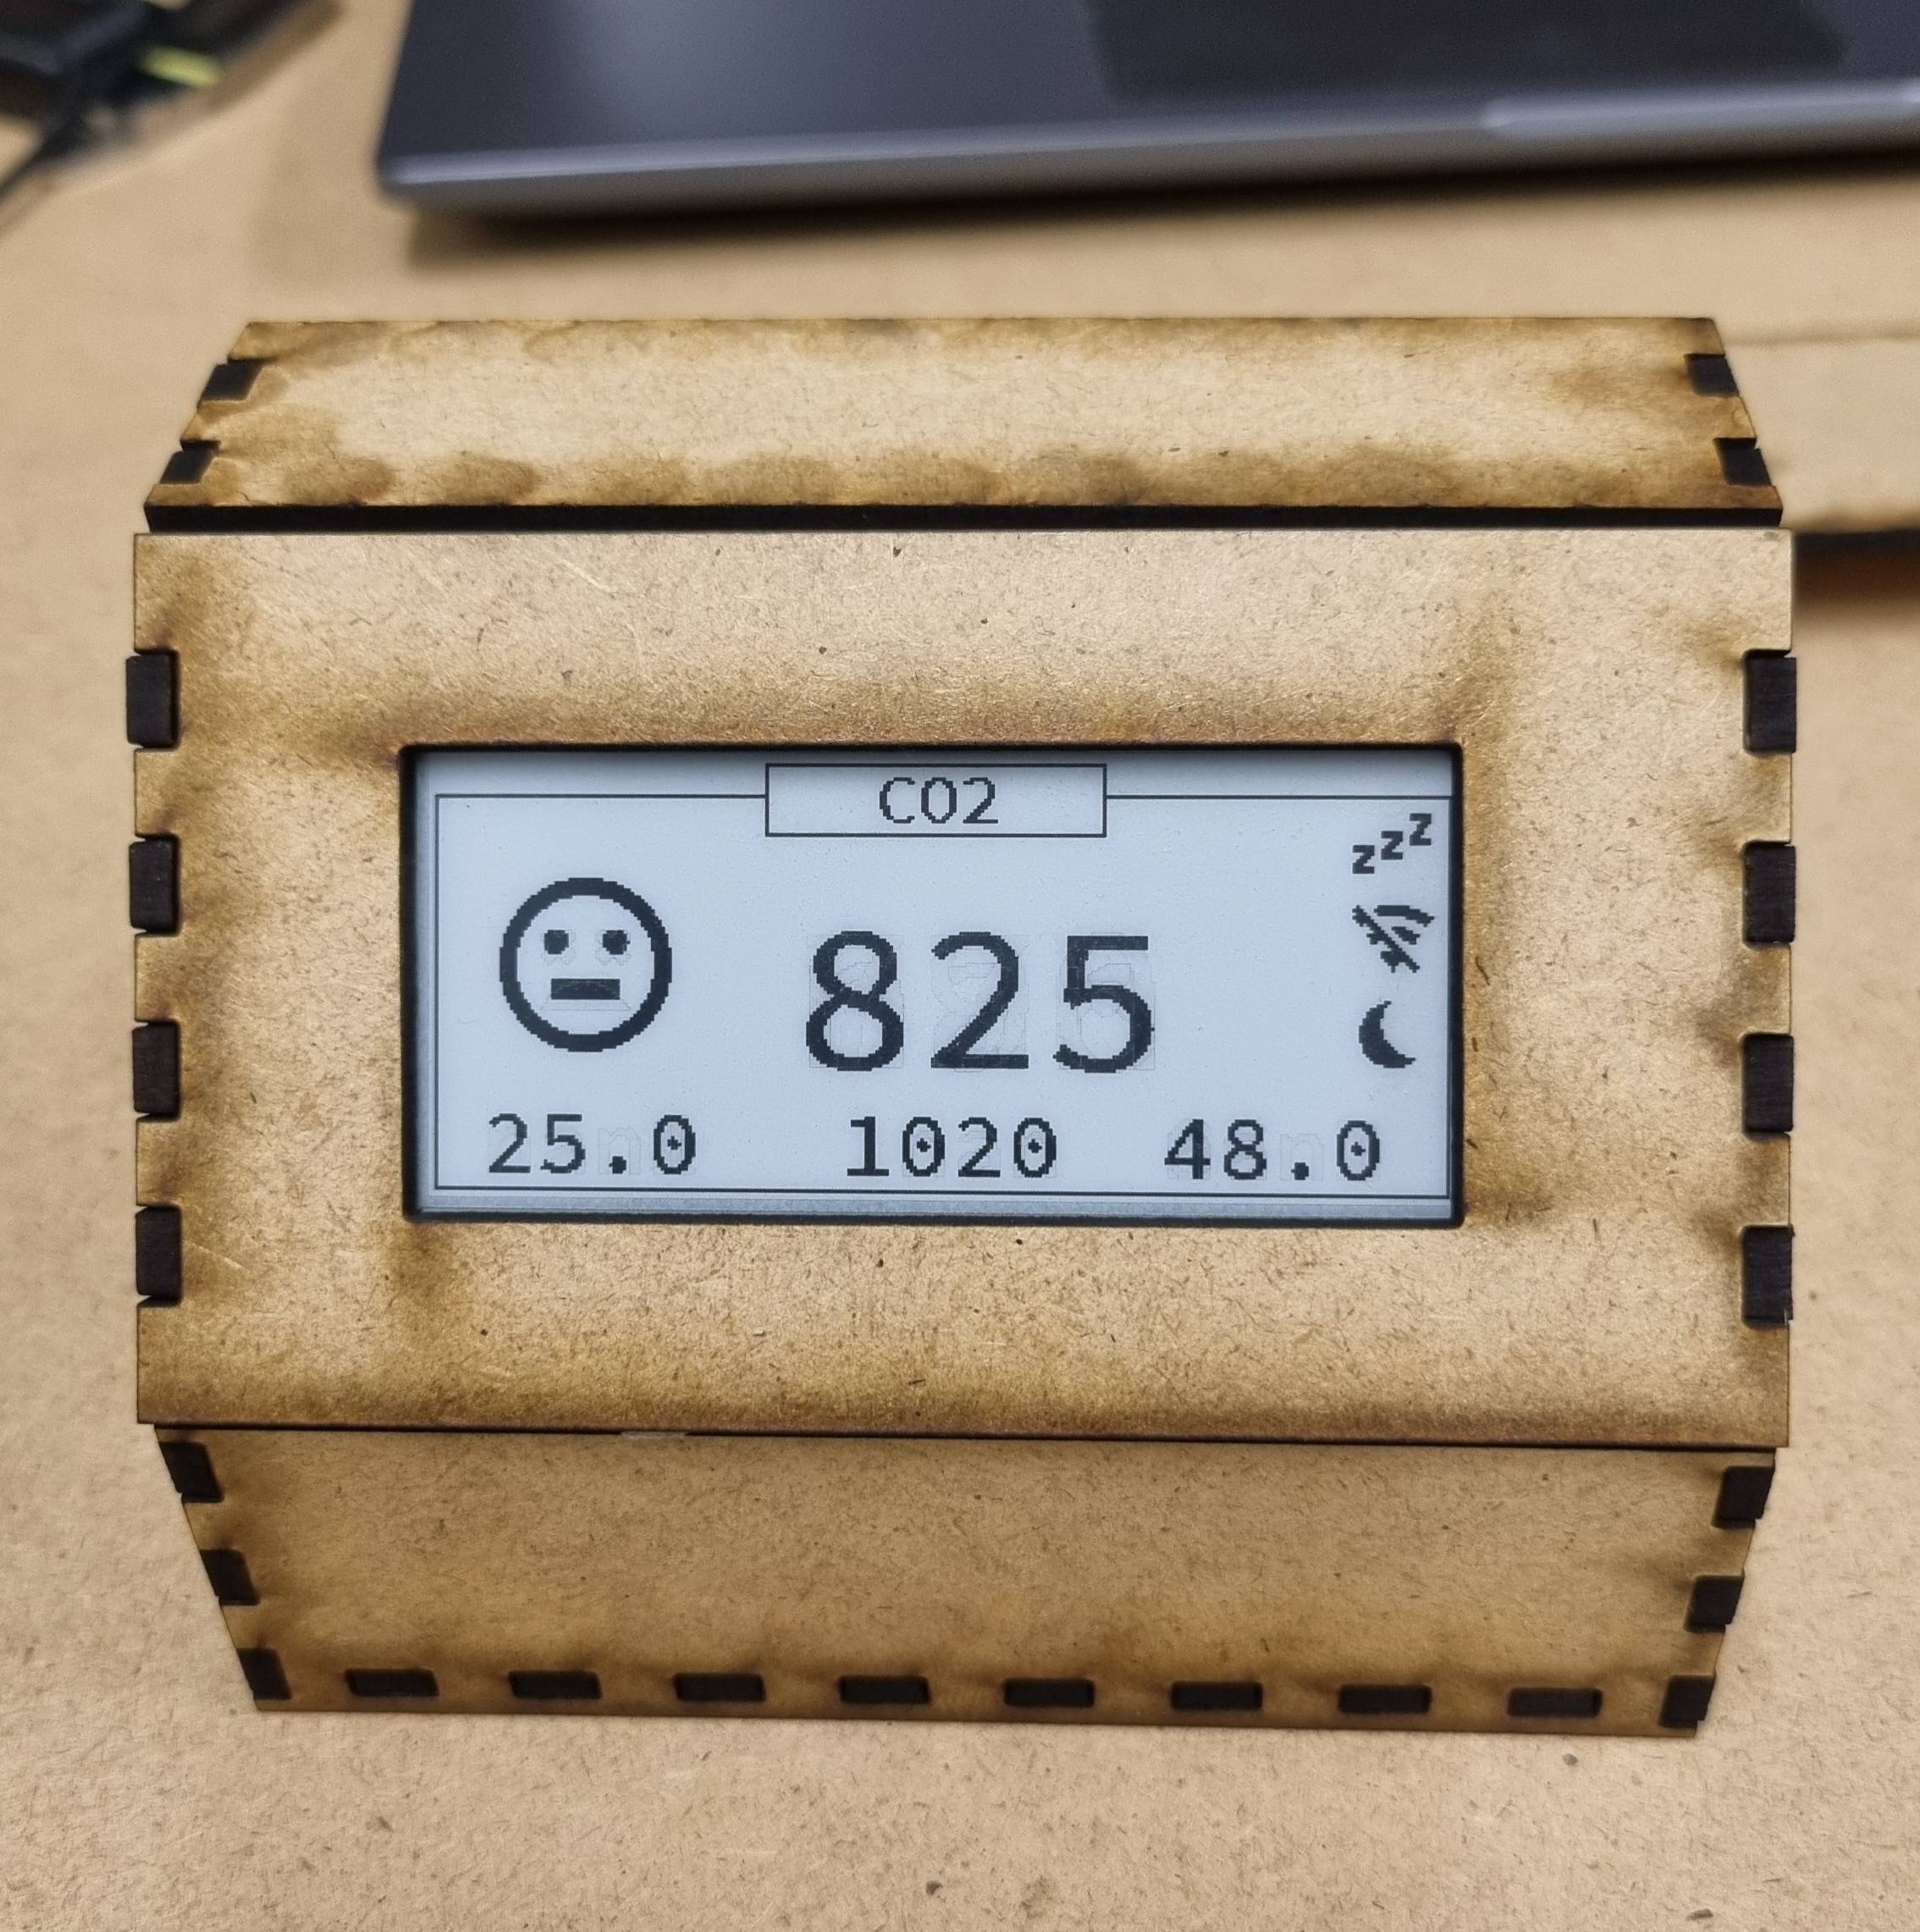
\includegraphics[height=0.9\textheight]{sensor-fertig-01.jpg}
\end{frame}

% \section{Motivation}
% \divider{\insertsection}
\begin{frame}%[<+->] %%Eine Folie
    \frametitle{Warum hab ich das gemacht?} %%Folientitel
    \begin{itemize}[<+->]
        \item Covid is not over
        \item Aranet ist teuer
        \item Das Display lag seit Jahren ungenutzt in einer Box
        \item Ich wollte sehen, ob ich das kann
    \end{itemize}
\end{frame}

\begin{frame}
    \frametitle{Inspiration}
    \begin{columns}[c]
        \begin{column}{0.5\textwidth}
            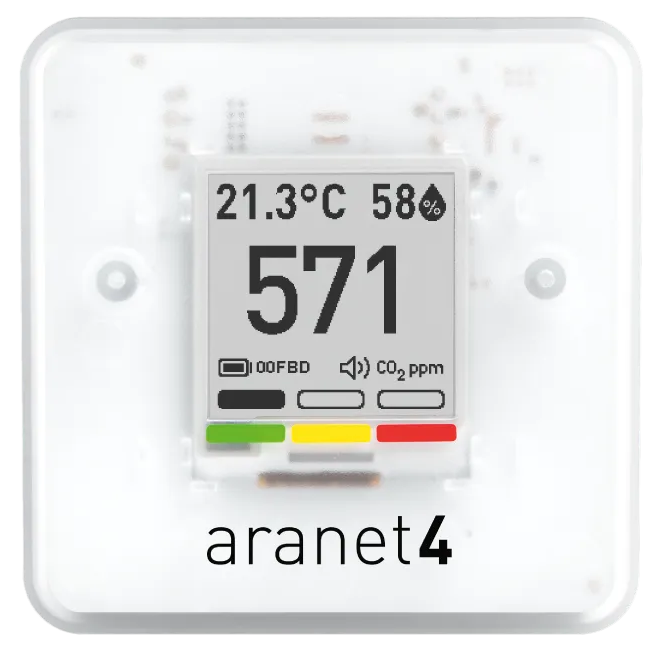
\includegraphics[width=0.8\textwidth]{Aranet4.png}\\
            Aranet HOME4
        \end{column}        
        % \pause
        \begin{column}{0.5\textwidth}
            \visible<2>{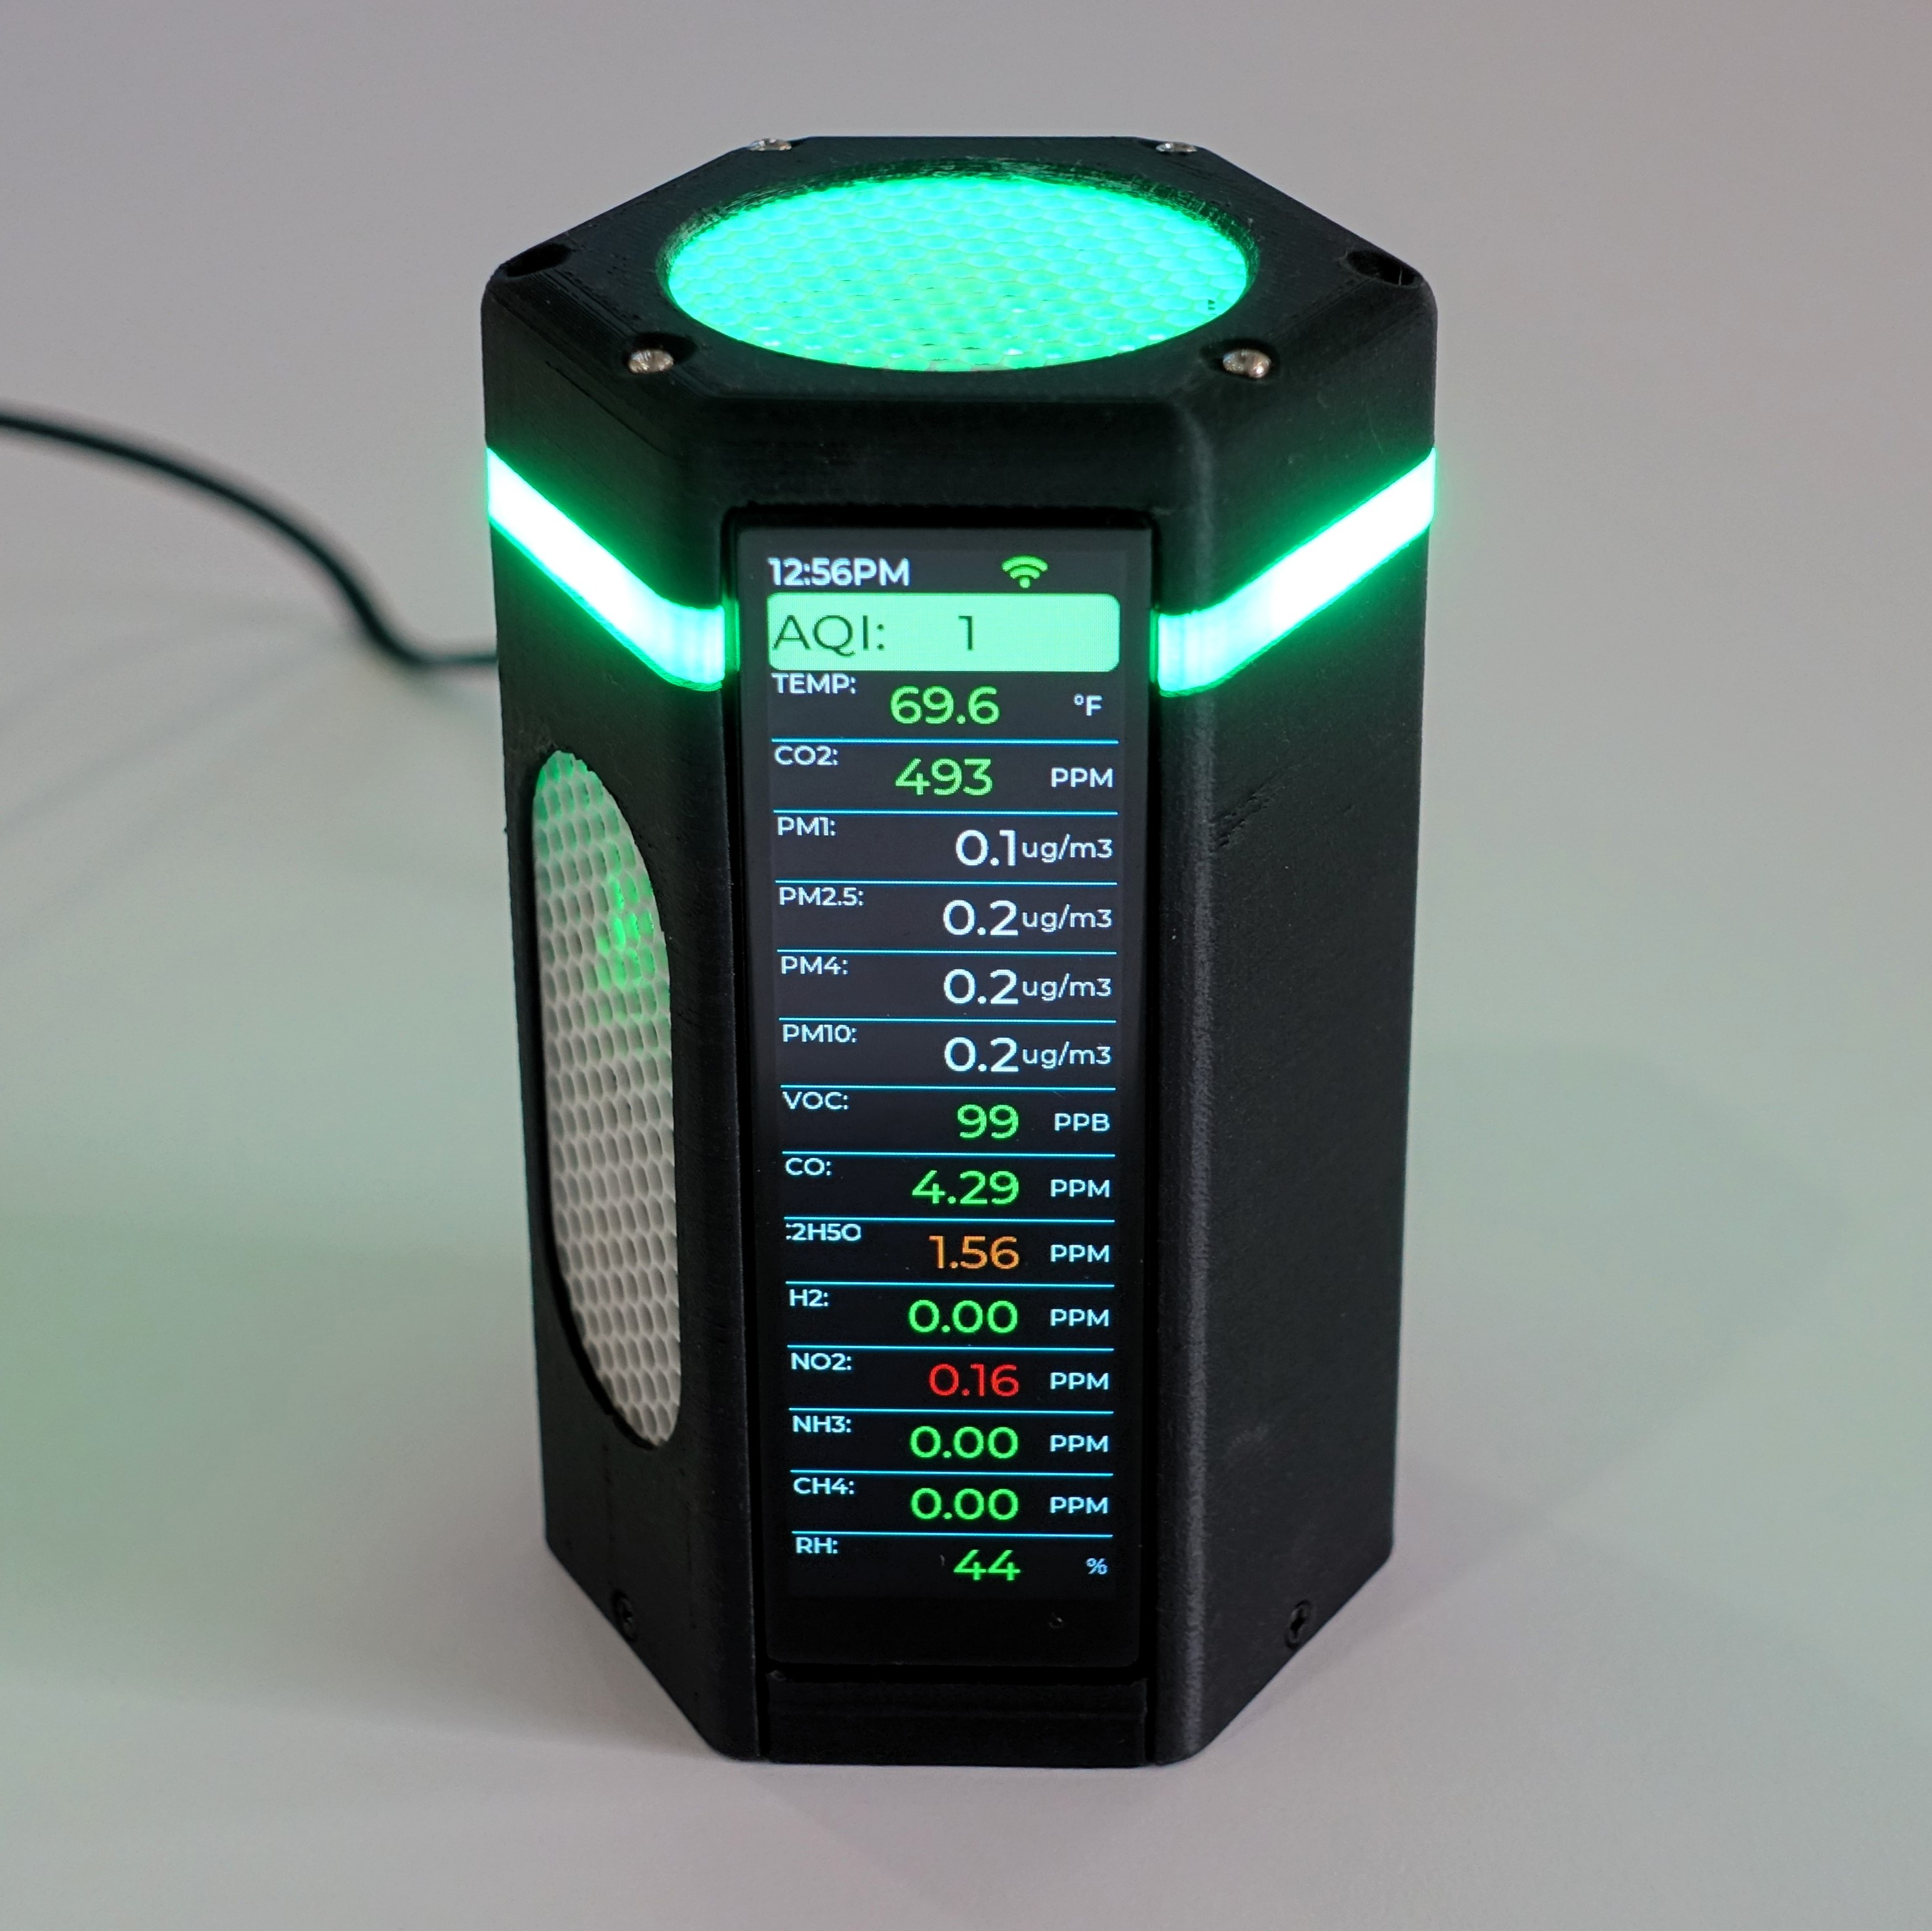
\includegraphics[width=0.8\textwidth]{Halo_v1.JPG}\\
            Halo by Yash Mulgaonkar}
        \end{column}
    \end{columns}
\end{frame}

\begin{frame}%[<+->] %%Eine Folie
    \frametitle{Die Bauteile} %%Folientitel
    \centering
    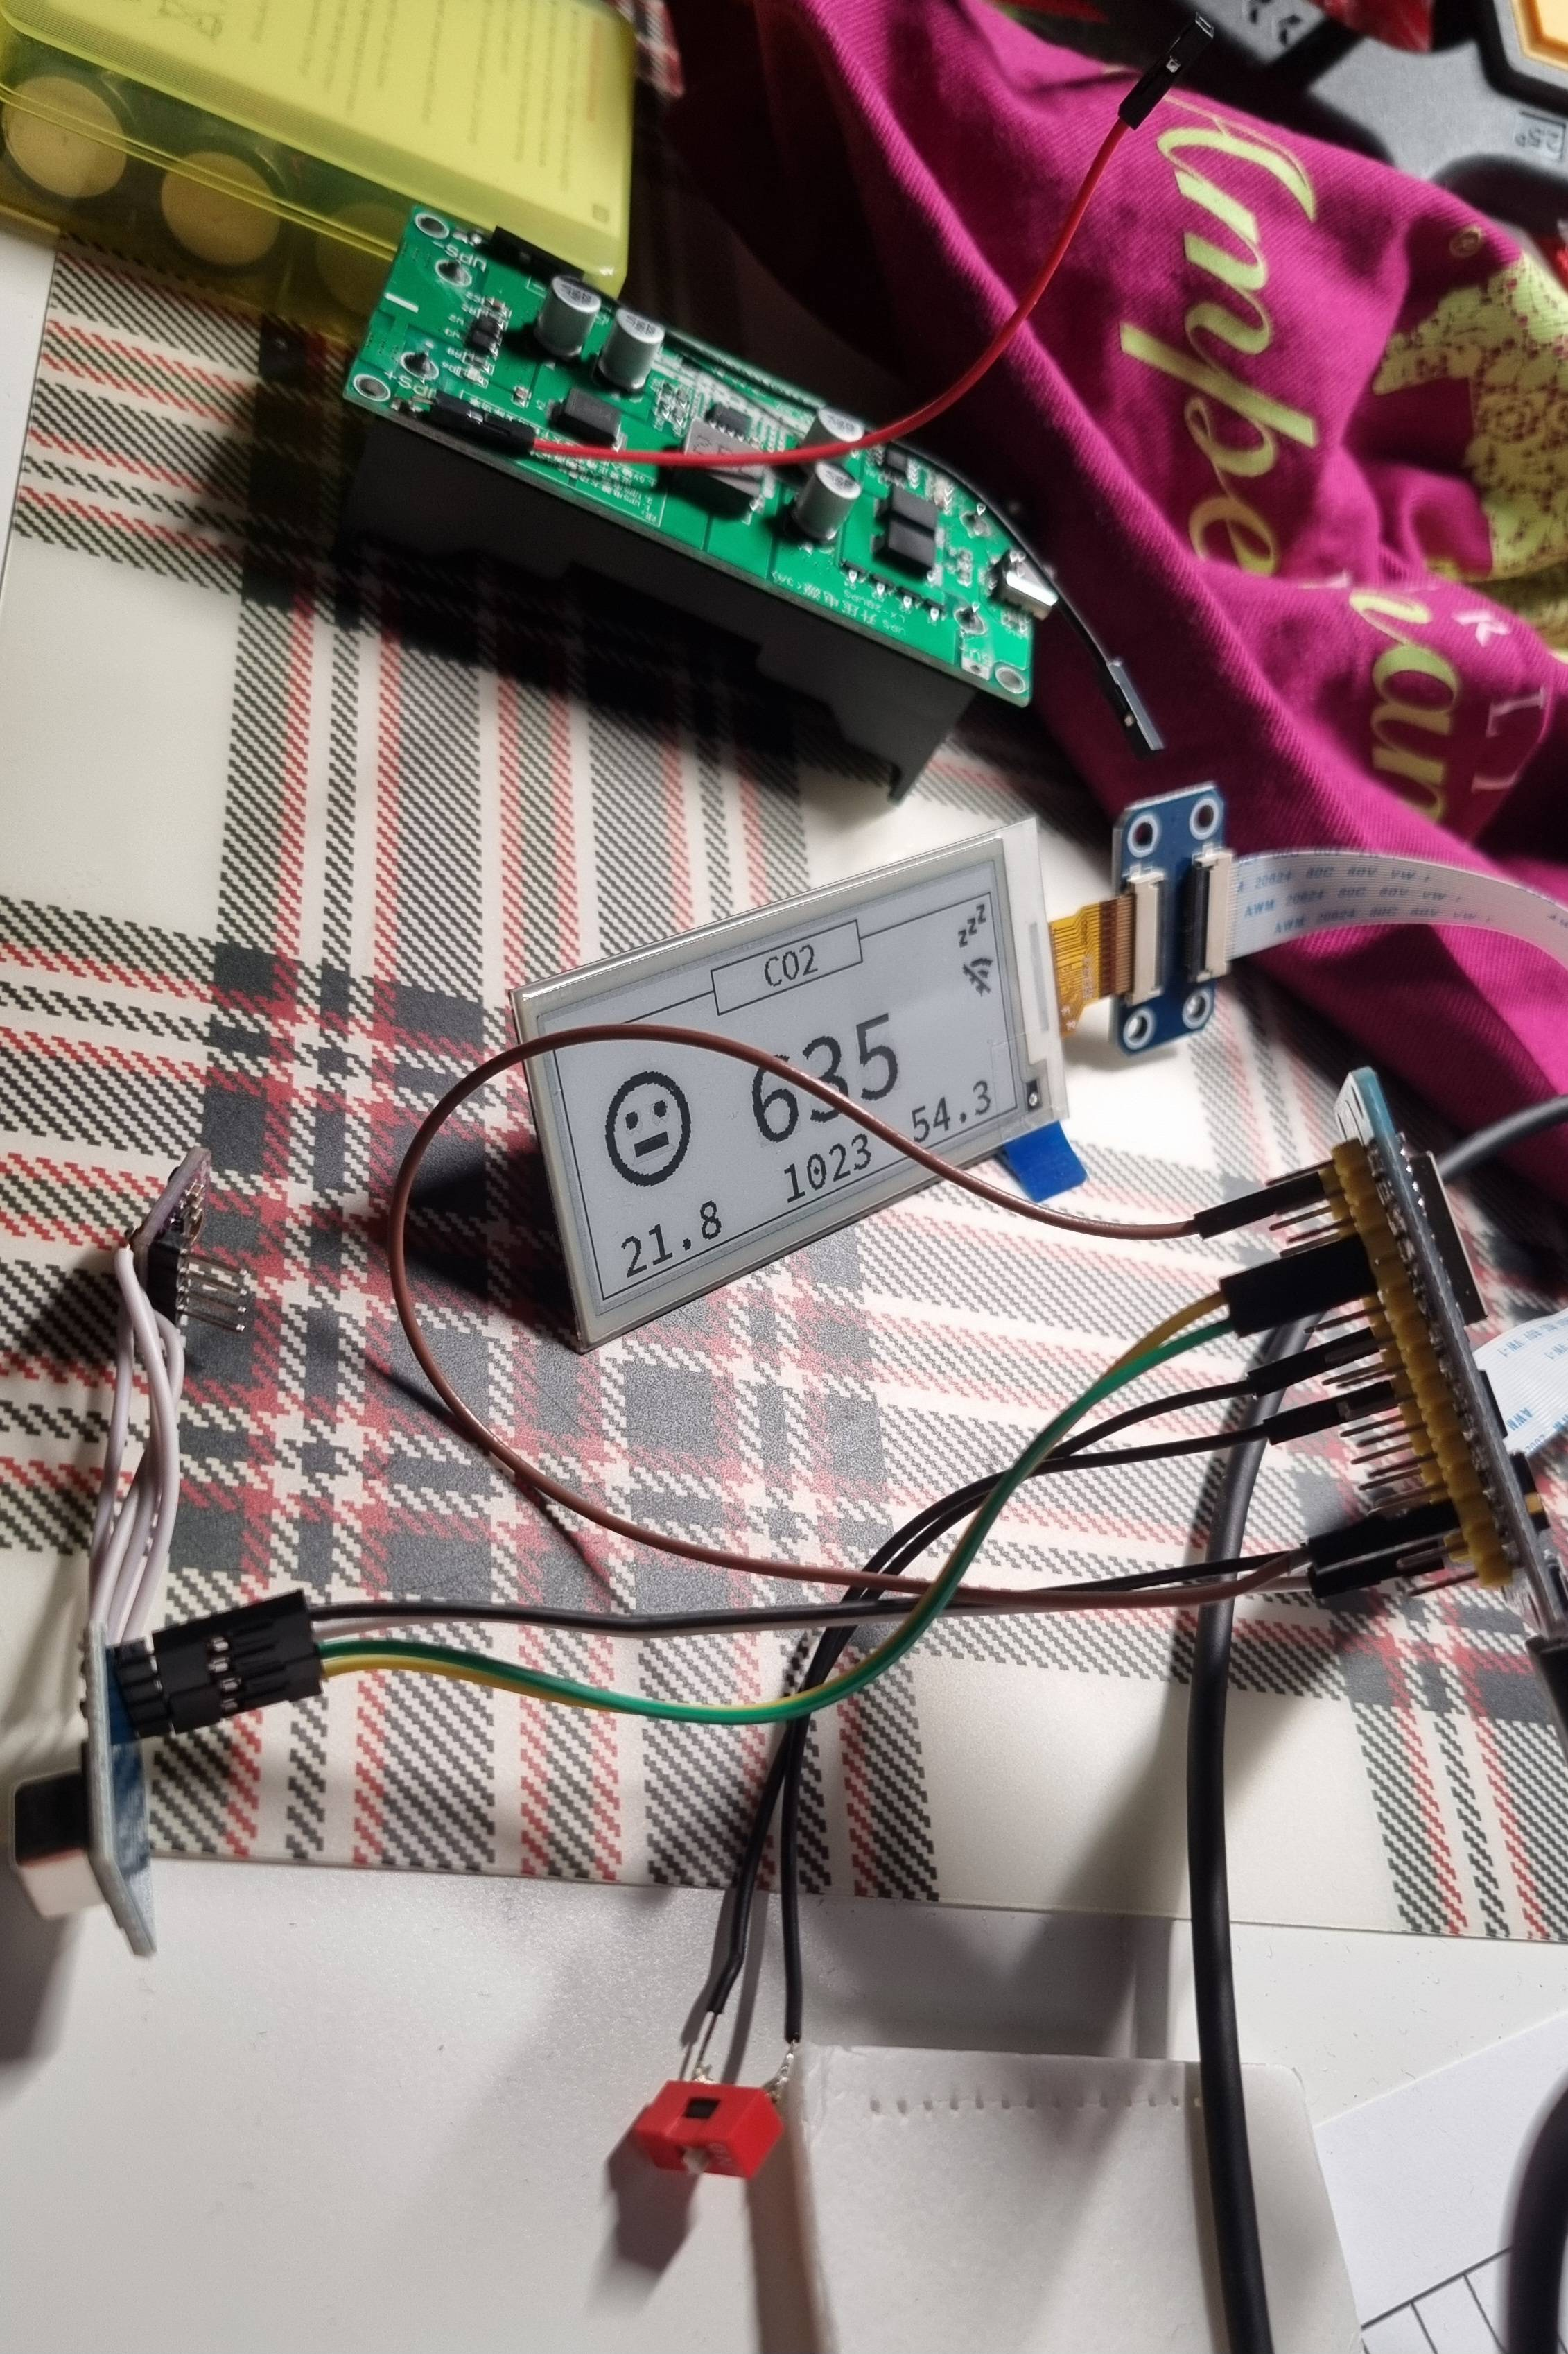
\includegraphics[width=0.9\textheight,angle=90]{bauteile-01.jpg}
\end{frame}

\begin{frame}%[<+->] %%Eine Folie
    \frametitle{Die Bauteile} %%Folientitel
    \begin{description}[<+->][labelwidth=20en]
       \item[Display] Waveshare \SI{2.9}{\inch} ePaper
       \item[Mikrocontroller] ESP8266
       \item[CO2 Sensor] SCD40
       \item[Zusatzsensor] BME280 (\si{\celsius}, \si{\hecto\pascal}, \%RH)
       \item[Akkucontroller] USB-C 18650 Controller von AliExpress
    \end{description}
\end{frame}

\begin{frame}
    \frametitle{Programmierung mit ESPHome}
    \begin{itemize}[<+->]
        \item Add-On von Home Assistant
        \item Konfiguration per YAML
        \item erzeugt C++ Code und kompiliert mit Arudino-Platform
    \end{itemize}
\end{frame}

\begin{frame}[fragile]
    \frametitle{CO2 Sensor}
    \footnotesize
\begin{lstlisting}[language=yaml]
sensor:
#SDC40 CO2 Sensor
  - platform: scd4x
    id: scd40
    co2:
      name: "Mobile CO2"
      id: sensorco2                                                              
    automatic_self_calibration: false
    update_interval: 10s
    measurement_mode: "periodic"
    i2c_id: esp_i2c
    ambient_pressure_compensation_source: sensorpressure
\end{lstlisting}
\end{frame}

\begin{frame}[fragile]
    \frametitle{Display}
    \footnotesize
\begin{lstlisting}[language=yaml]
# Configure e-ink display
display:
  - platform: waveshare_epaper
    cs_pin: 15 #D8
    dc_pin: 4 #D2
    reset_pin: 5 #D1
    model: 2.90in #296x128 pixels
    rotation: 90
    update_interval: 10s
    lambda: |-
      // Rahmen zeichnen und Ueberschrift schreiben
      it.rectangle(2, 12, it.get_width()-4, it.get_height()-14);
      it.filled_rectangle(it.get_width()/3, 11, it.get_width()/3, 3, COLOR_OFF);
      it.rectangle(it.get_width()/3, 3, it.get_width()/3, 21);
      it.print(it.get_width()/2, 0, id(fontText), TextAlign::TOP_CENTER, "CO2");
      // CO2 Messwert schreiben
      it.printf(70, 30, id(fontMainValue), "%4.0f", id(sensorco2).state);
\end{lstlisting}
\end{frame}

\begin{frame}[fragile]
    \frametitle{Fonts und Symbole}
    \footnotesize
\begin{lstlisting}[language=yaml]
# Fonts
font:
  - file: "materialdesignicons-webfont.ttf"
    id: iconsLarge
    size: 60
    glyphs: [
      "\U000F01F2", #mdi emoticon happy
      "\U000F01F6", #mdi emoticon neutral
      "\U000F01F8", #mdi emoticon unhappy
      "\U000F069B", #mdi emoticon dead
      ]
\end{lstlisting}
\end{frame}

\begin{frame}[fragile]
    \frametitle{Emoji zeichnen}
    \footnotesize
\begin{lstlisting}[language=yaml]
      // Emote zeichnen, abhaengig vom CO2
      char emote[5];
      if (id(sensorco2).state < 600.0)
      {
        sprintf(emote, "\U000F01F2");
      }
      else if (id(sensorco2).state < 1000.0)
      {
        sprintf(emote, "\U000F01F6");
      }
      else if (id(sensorco2).state < 1500.0)
      {
        sprintf(emote, "\U000F01F8");
      }
      else
      {
        sprintf(emote, "\U000F069B");
      }
      it.print(16, 30, id(iconsLarge), emote);
\end{lstlisting}
\end{frame}

\begin{frame}
    \frametitle{Extra Features}
    \begin{itemize}[<+->]
        \item Deep Sleep: \SI{2}{\minute} schlafen, \SI{1}{\minute} wach
        \item Always On Modus umschaltbar mit Schalter
    \end{itemize}
\end{frame}

\begin{frame}
    \frametitle{Gehäuse}
    \texttt{boxes.py} to the rescue!\\
    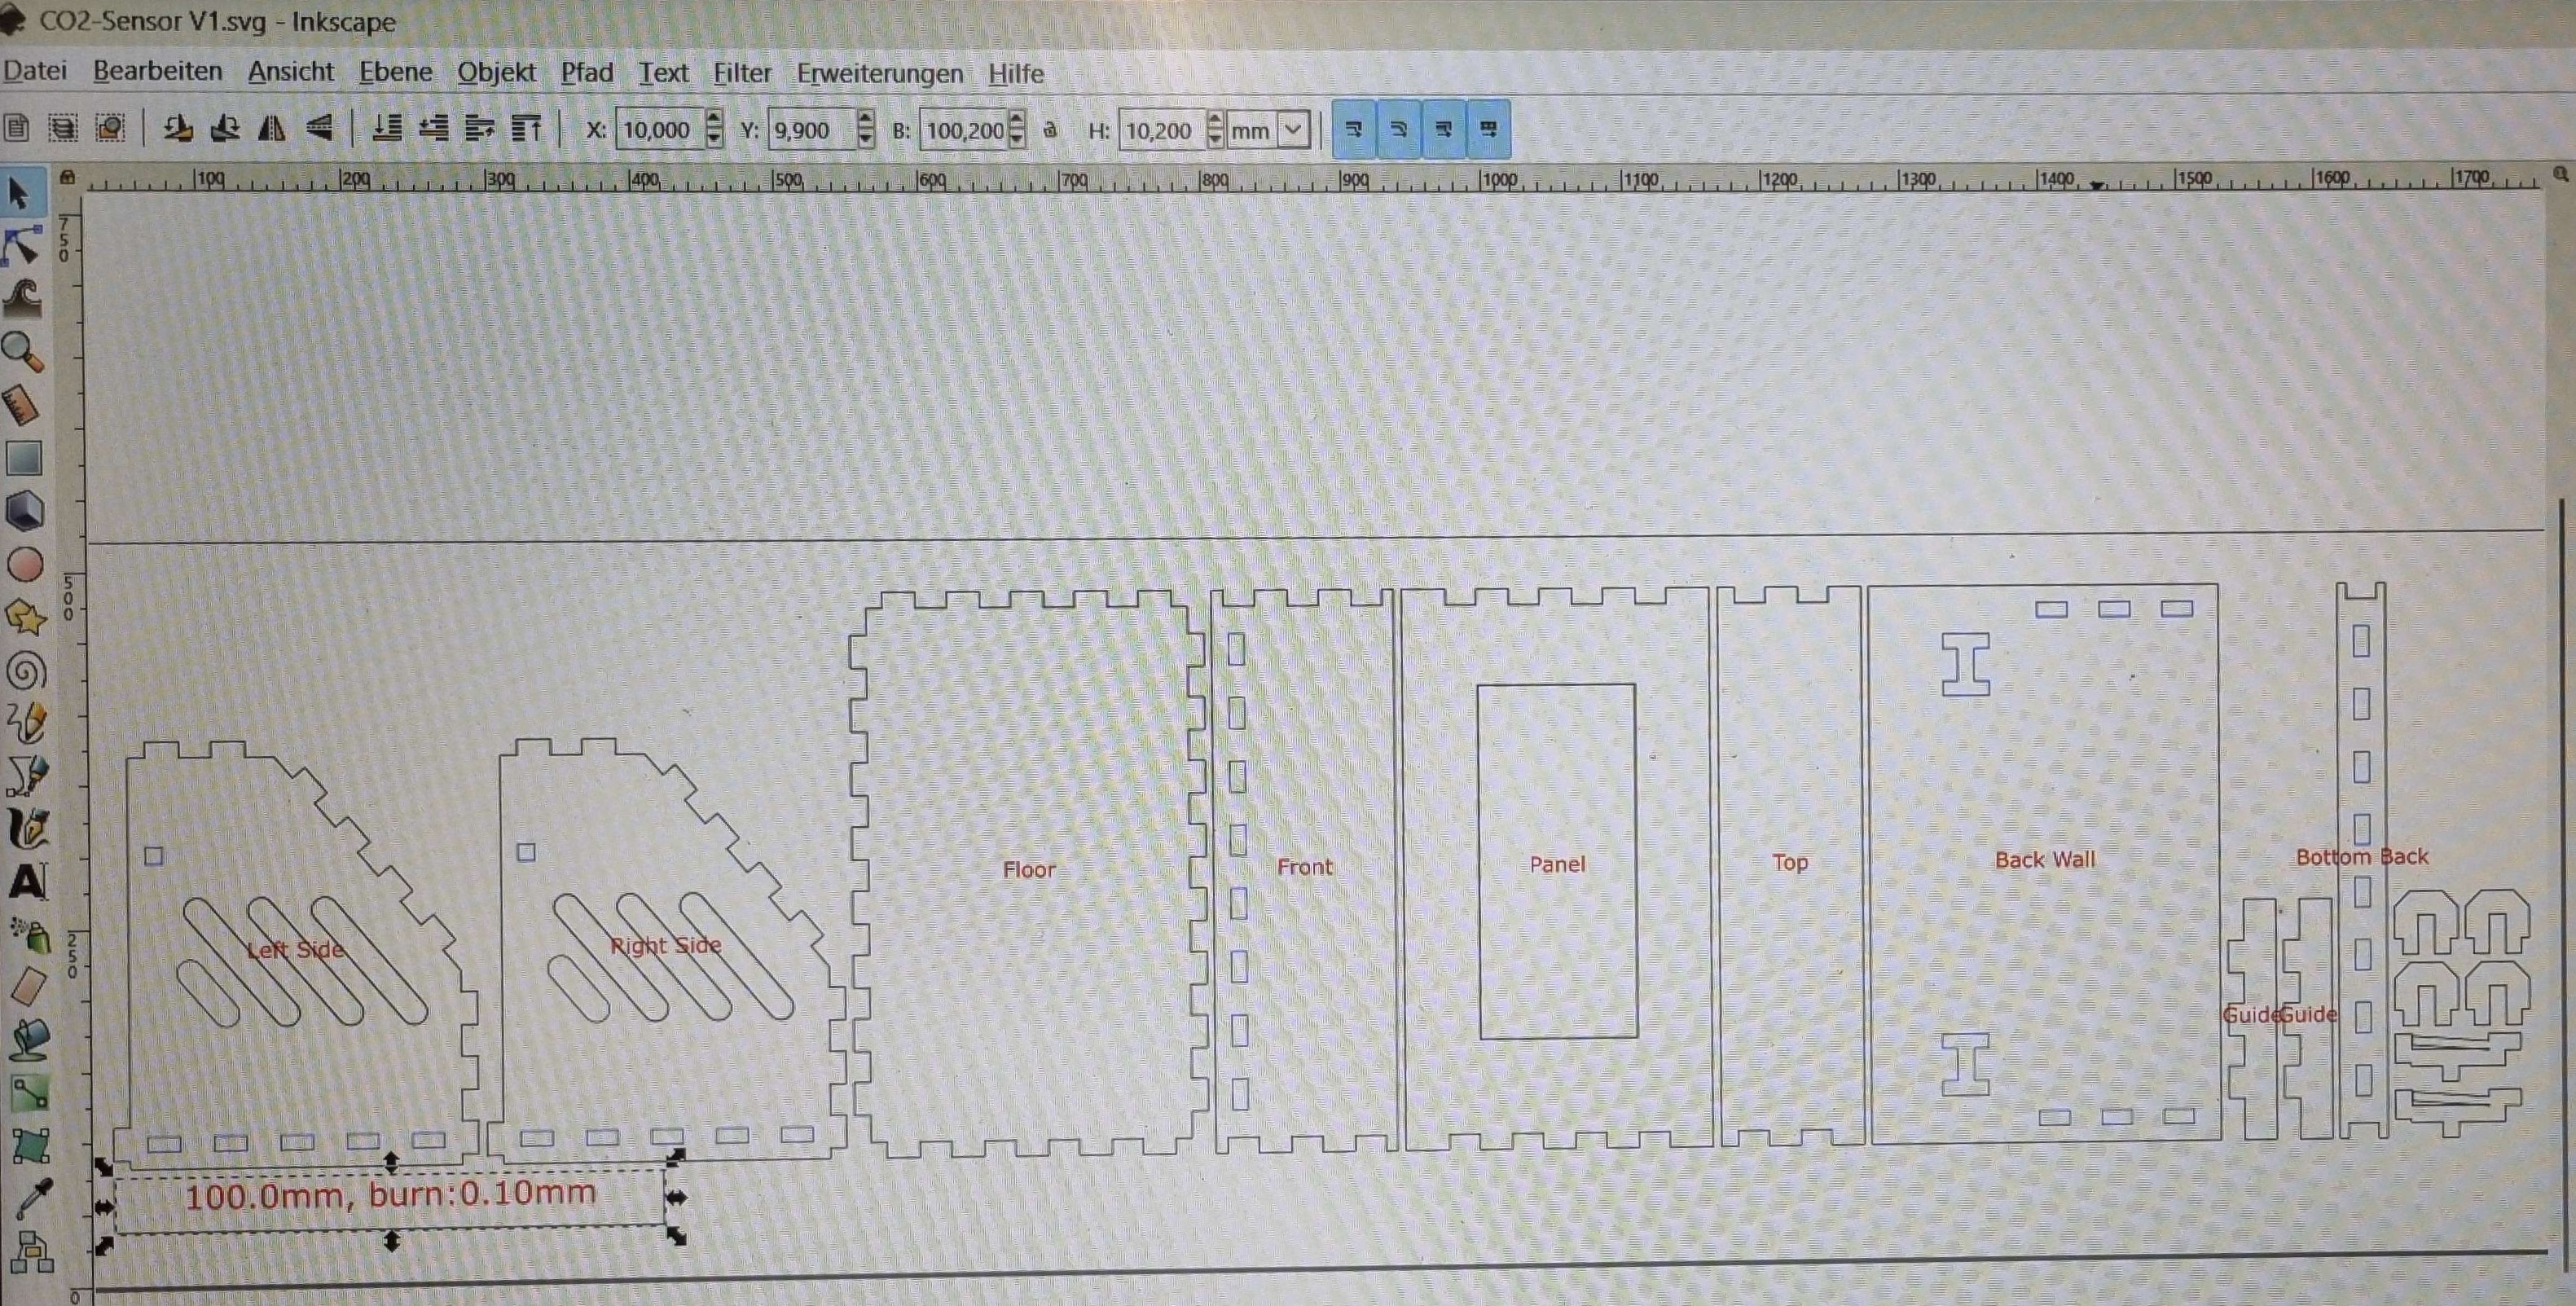
\includegraphics[height=0.8\textheight]{boxes-py-02.jpg}
\end{frame}

\begin{frame}
    \frametitle{Gehäuse}
    \enquote{Laser}\\
    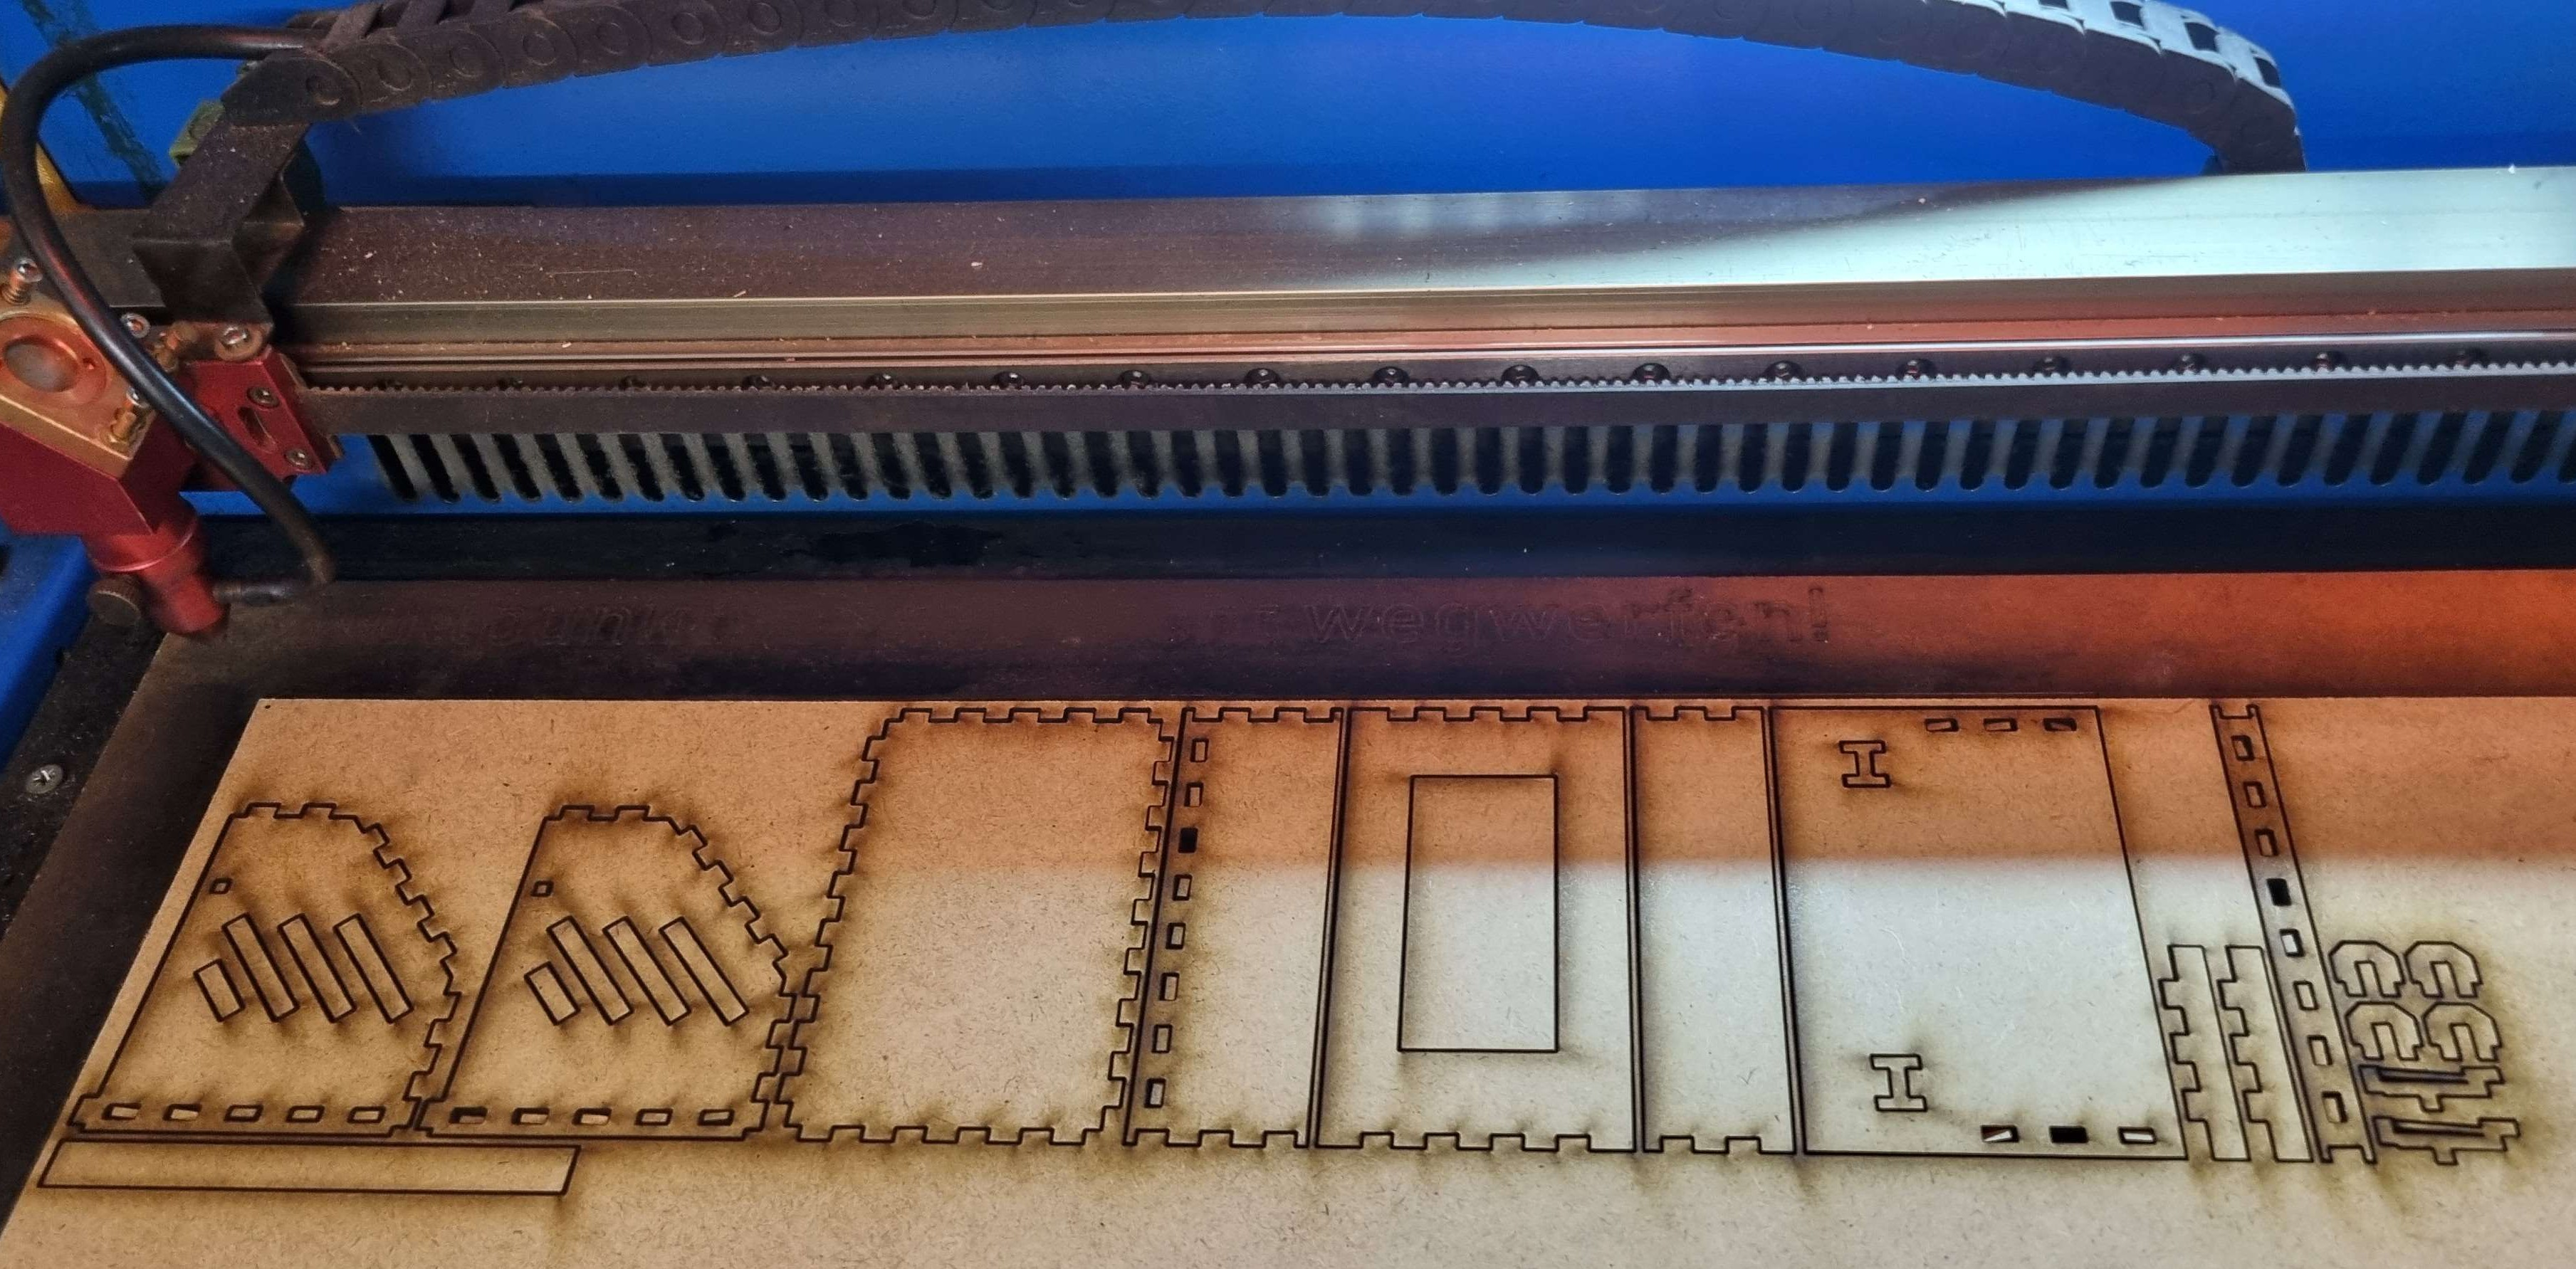
\includegraphics[height=0.8\textheight]{laser-02.jpg}
\end{frame}

\begin{frame}
    \frametitle{Danke für die Aufmerksamkeit!}
    @syralist@troet.cafe\\
    DECT 7972\\
    \href{https:\\syralist.de}{syralist.de}
\end{frame}

\end{document}